%----------------------------------------------------------------------------------------
%	PACKAGES AND THEMES
%----------------------------------------------------------------------------------------
\documentclass[aspectratio=169,xcolor=dvipsnames]{beamer}
% \usetheme{SimplePlus}

\usepackage{hyperref}
\usepackage{graphicx} % Allows including images
\usepackage{booktabs} % Allows the use of \toprule, \midrule and \bottomrule in tables

%----------------------------------------------------------------------------------------
%	TITLE PAGE
%----------------------------------------------------------------------------------------

\title[short title]{Enhancing CHIM-XPT} % The short title appears at the bottom of every slide, the full title is only on the title page
\subtitle{A Geochemical Modeling Tool for Mars Research}

\author[Nikaansh Singh] {Nikaansh Singh}

\institute[PSU] % Your institution as it will appear on the bottom of every slide, may be shorthand to save space
{
    Institute for Computing in Research \\
    Portland State University % Your institution for the title page
}
\date{\today} % Date, can be changed to a custom date


%----------------------------------------------------------------------------------------
%	PRESENTATION SLIDES
%----------------------------------------------------------------------------------------

\begin{document}

\begin{frame}
    % Print the title page as the first slide
    \titlepage
\end{frame}

%------------------------------------------------
\section{First Section}
%------------------------------------------------

\begin{frame}{Ice Caps and Water on Mars}
\begin{figure}
    \centering
    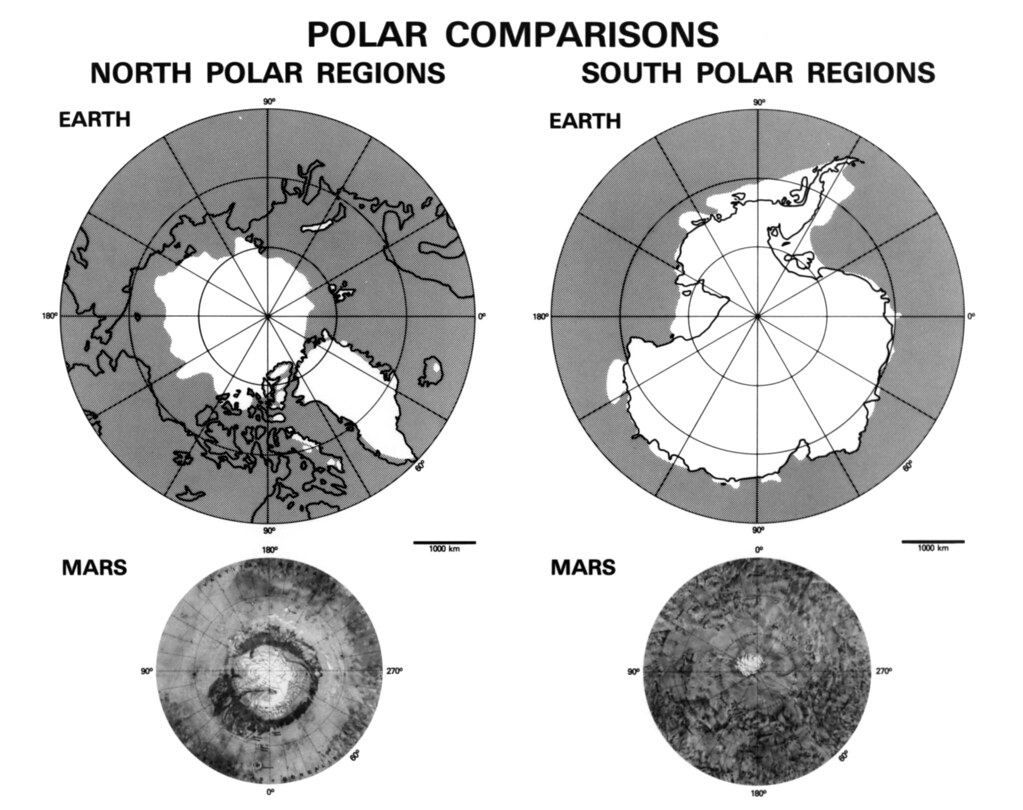
\includegraphics[width=0.5\linewidth]{ice-caps.png}
    \caption{Composition of Earth's and Mar's Ice Caps  (Lunar and Planetary Institute, 2009)}
    \label{fig:enter-label}
\end{figure}
\end{frame}

%------------------------------------------------

\begin{frame}{How is CHIM-XPT Used}
    CHIM-XPT is run through the use of the \alert{terminal and editing files}. When having the run hundreds of trials with outputs that can get in the tens of thousands, this can get tiring

\begin{figure}
    \centering
    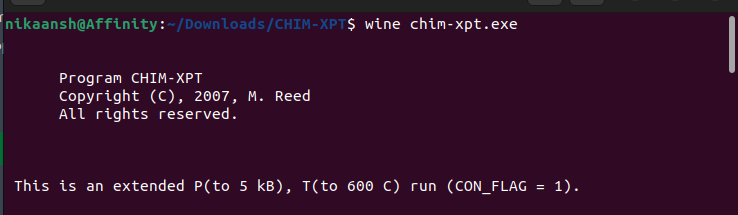
\includegraphics[width=1\linewidth]{screenshot1.png}
    \caption{Running CHIM-XPT in Terminal Using Wine}
    \label{fig:enter-label}
\end{figure}
\end{frame}

%------------------------------------------------

\begin{frame}{How is CHIM-XPT Used Cont.}
    \begin{columns}[c] % The "c" option specifies centered vertical alignment while the "t" option is used for top vertical alignment

        \column{.45\textwidth} % Left column and width
        \textbf{Files}
        \begin{enumerate}
            \item CHIMRUN.DAT
            \item CHIMOUT.DAT
            \item CHIMPLOT.DAT
            \item CHIMTERMINAL.DAT
        \end{enumerate}

        \column{.5\textwidth} % Right column and width
        \begin{figure}
            \centering
            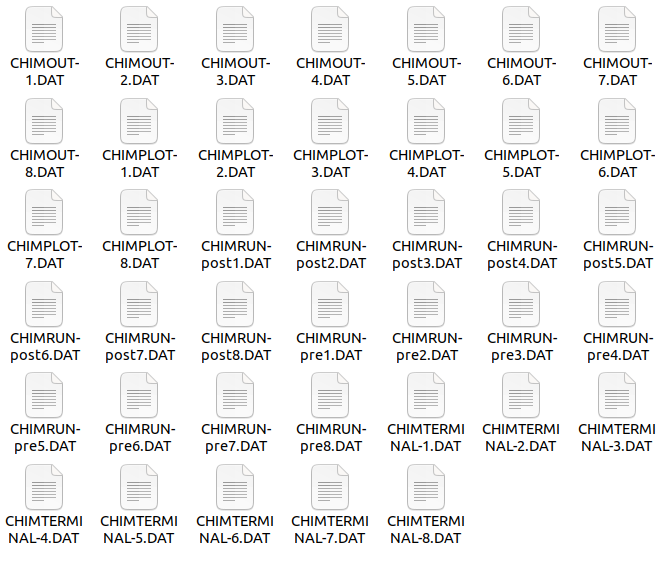
\includegraphics[width=1\linewidth]{screenshot2.png}
            \caption{File Output after Running CHIM-XPT}
            \label{fig:enter-label}
        \end{figure}
        
    \end{columns}
\end{frame}

%------------------------------------------------
\section{Second Section}
%------------------------------------------------

\begin{frame}{CHIMRUN Data}
    \begin{columns}[c] % The "c" option specifies centered vertical alignment while the "t" option is used for top vertical alignment

        \column{.45\textwidth} % Left column and width
        \textbf{Data}
        \begin{enumerate}
            \item ph/pFluid/Temp
            \item Stem Limit/Increm
            \item Mineral Suppress List
        \end{enumerate}

        \column{.5\textwidth} % Right column and width
        \begin{figure}
            \centering
            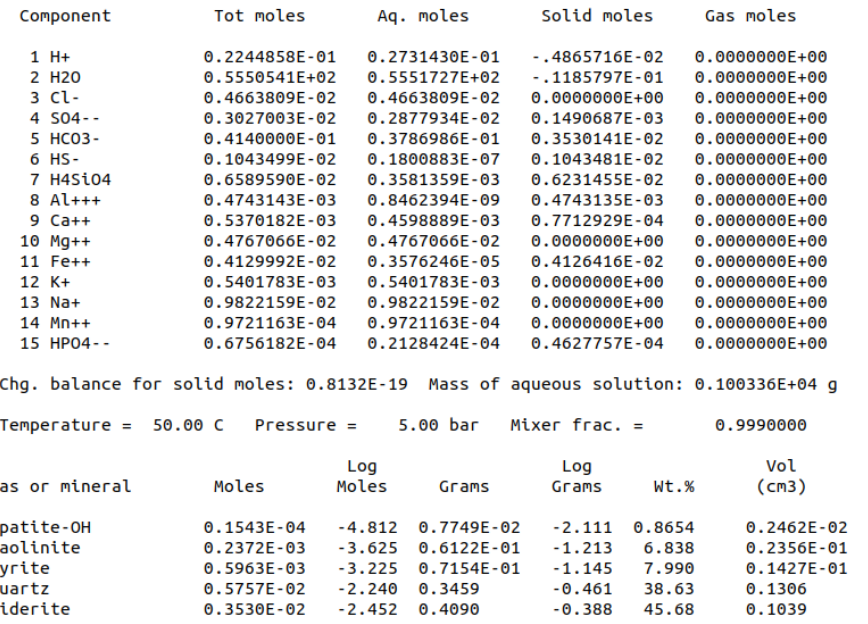
\includegraphics[width=1\linewidth]{screenshot3.png}
            \caption{Data from CHIMRUN}
            \label{fig:enter-label}
        \end{figure}
        
    \end{columns}
\end{frame}

%------------------------------------------------

\begin{frame}{CHIMOUT Data}
    \begin{table}
        \begin{tabular}{l l l}
            \toprule
            \textbf{Name} & \textbf{Log(Water/Rock)} & \textbf{Weight Percentage} \\
            \midrule
            kaolinite & 2.0015 & 6.838    \\
            pyrite & 2.0015 & 7.990       \\
            quartz & 2.0015 & 38.63       \\
            siderite & 2.0015 & 45.68     \\
            \bottomrule
        \end{tabular}
        \caption{Example data from CHIMOUT}
    \end{table}
\end{frame}

%------------------------------------------------

\begin{frame}{CHIMOUT Data Cont.}
    \begin{figure}
        \centering
        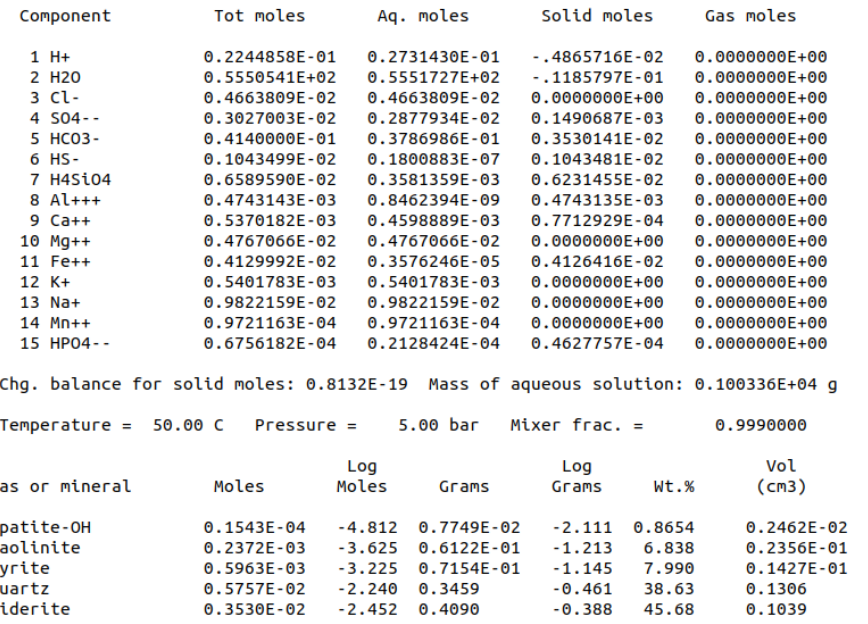
\includegraphics[width=0.7\linewidth]{screenshot3.png}
        \caption{Data from CHIMRUN}
        \label{fig:enter-label}
    \end{figure}
\end{frame}

%------------------------------------------------

\begin{frame}{CHIMTERMINAL Data}
    \begin{columns}[c] % The "c" option specifies centered vertical alignment while the "t" option is used for top vertical alignment

        \column{.45\textwidth} % Left column and width
        \textbf{Data}
        \begin{enumerate}
            \item Ionic Strength
            \item Weight Percentage
            \item pH
            \item Errors
        \end{enumerate}

        \column{.5\textwidth} % Right column and width
        \begin{figure}
            \centering
            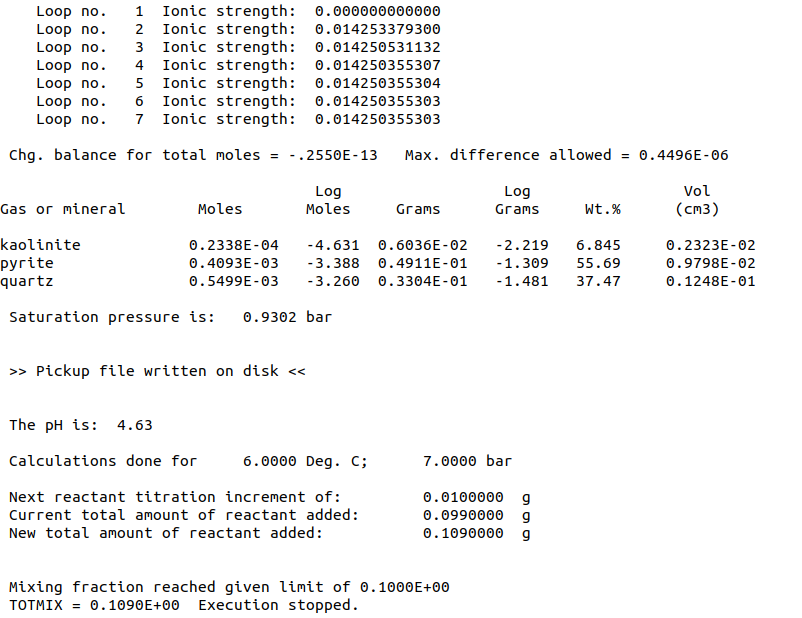
\includegraphics[width=1\linewidth]{screenshot4.png}
            \caption{Data from CHIMTERMINAL}
            \label{fig:enter-label}
        \end{figure}
        
    \end{columns}
\end{frame}

%------------------------------------------------

\begin{frame}{CHIMPLOT Data}
    \begin{figure}
        \centering
        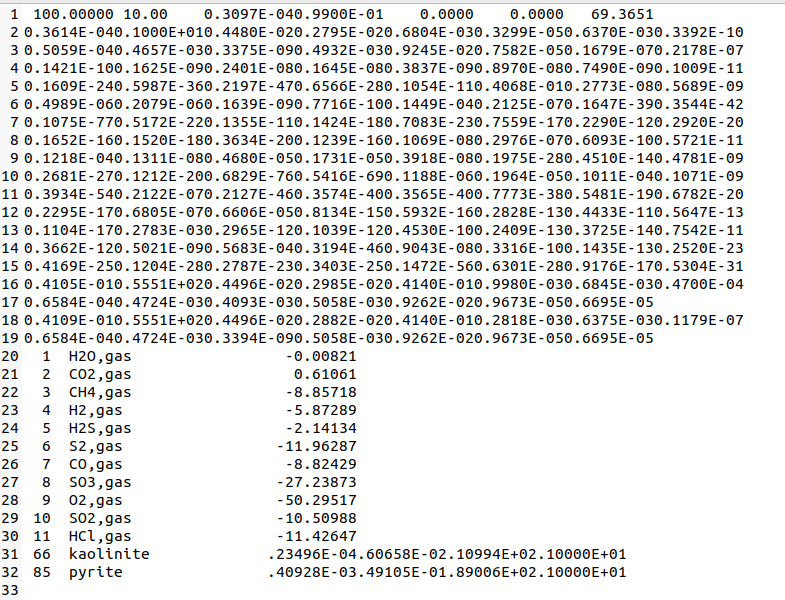
\includegraphics[width=0.6\linewidth]{Screenshot5.png}
        \caption{Data from CHIMPLOT}
        \label{fig:enter-label}
    \end{figure}
\end{frame}

%------------------------------------------------

\begin{frame}{}
    \begin{figure}
        \centering
        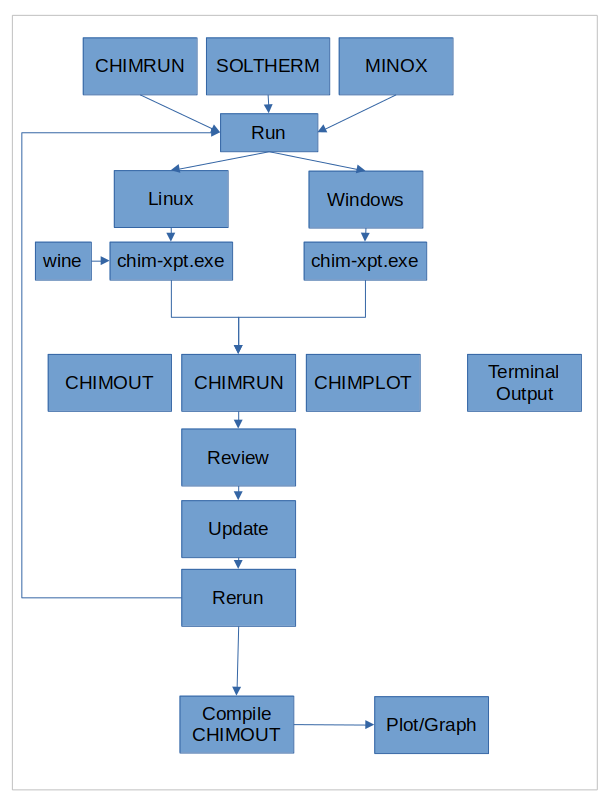
\includegraphics[width=0.48\linewidth]{image.png}
        \label{fig:enter-label}
    \end{figure}
\end{frame}

%------------------------------------------------

\begin{frame}{CHIM-XPT Wrapper}
    \begin{figure}
        \centering
        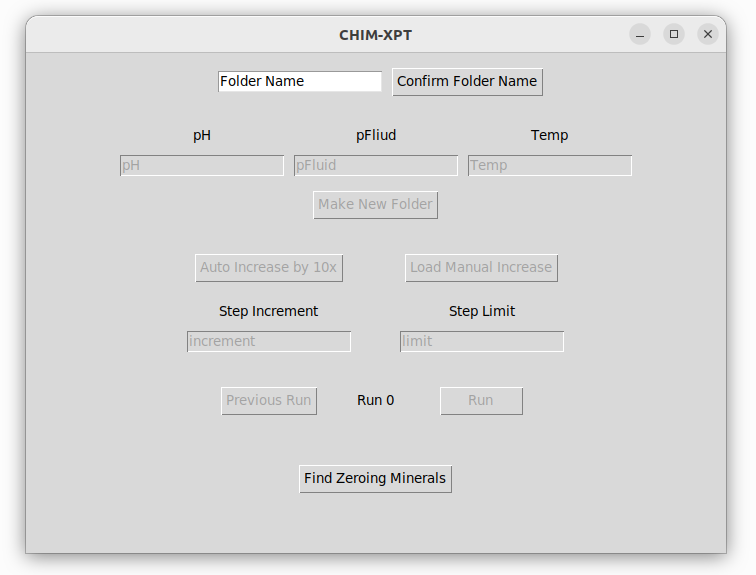
\includegraphics[width=0.6\linewidth]{chim.png}
        \caption{Picture of GUI Created after Running my CHIM Wrapper}
        \label{fig:enter-label}
    \end{figure}
\end{frame}

%------------------------------------------------

\begin{frame}{Graphing GUI}
    \begin{figure}
        \centering
        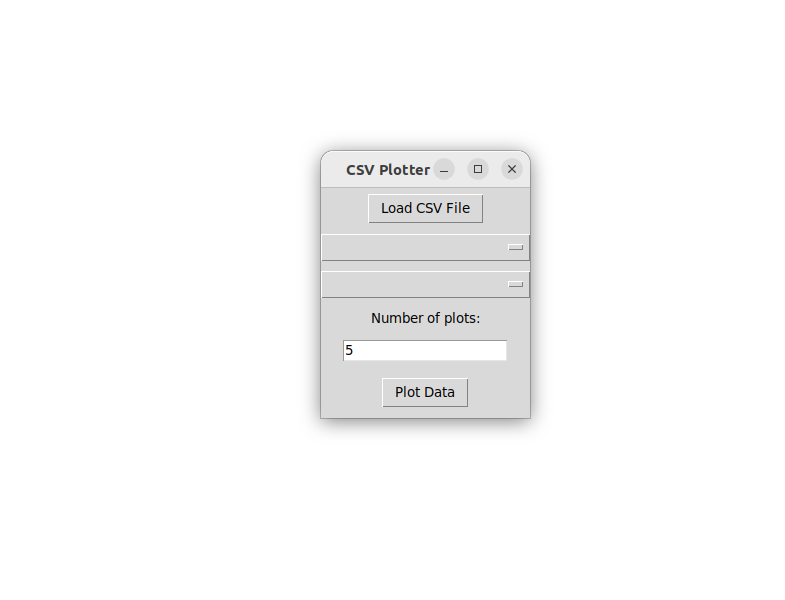
\includegraphics[width=0.6\linewidth]{graph.png}
        \caption{GUI Created after Running my Graphing Program}
        \label{fig:enter-label}
    \end{figure}
\end{frame}

%------------------------------------------------
\begin{frame}{Challenges and Future Steps}
    \begin{columns}[c] % The "c" option specifies centered vertical alignment while the "t" option is used for top vertical alignment

    \column{.45\textwidth} % Left column and width
        \textbf{Challenges}
        \begin{enumerate}
            \item Running Windows Executable
            \item No Access to Source Files
            \item Varying Columns and Headers
    \end{enumerate}

    \column{.5\textwidth} % Left column and width
        \textbf{Future Steps}
        \begin{enumerate}
            \item Combine the two GUIs
            \item Add a More Efficient Error Recovery
            \item Have a more Advanced Custom Graphing
        \end{enumerate}
        
    \end{columns}
\end{frame}

%------------------------------------------------

\begin{frame}
    \Huge{\centerline{\textbf{The End}}}
\end{frame}

%----------------------------------------------------------------------------------------

\end{document}
